% Created 2022-04-20 St 23:25
% Intended LaTeX compiler: pdflatex
\documentclass[11pt]{article}
\usepackage[utf8]{inputenc}
\usepackage[T1]{fontenc}
\usepackage{graphicx}
\usepackage{longtable}
\usepackage{wrapfig}
\usepackage{rotating}
\usepackage[normalem]{ulem}
\usepackage{amsmath}
\usepackage{amssymb}
\usepackage{capt-of}
\usepackage{hyperref}
\author{Andrej Zaujec}
\date{\today}
\title{BZA Project: Binary Reversing}
\hypersetup{
 pdfauthor={Andrej Zaujec},
 pdftitle={BZA Project: Binary Reversing},
 pdfkeywords={},
 pdfsubject={},
 pdfcreator={Emacs 28.0.50 (Org mode 9.6)}, 
 pdflang={English}}
\begin{document}

\maketitle
\tableofcontents


\section{Assigment}
\label{sec:orgdbb6f34}
Assigment of this project is to reverse engineer the three chosen binaries and propose the write-up of solutions, which are either from \href{https://hackthebox.com}{hackthebox} or the \href{https://crackmes.one/}{crackme}. The difficulty of these binaries should be medium or easy.
I did choose one binary from hackthebox and two others from crackme.
\begin{itemize}
\item \href{https://app.hackthebox.com/challenges/bombs-landed}{Bombs Landed:} had hard difficulty in time of reversing it and afterwards the difficulty was set to medium
\item \href{https://crackmes.one/crackme/5c2acb8933c5d46a3882b8d4}{Simple Keygen:} has easy diffuculty
\item \href{https://crackmes.one/crackme/5cfb961a33c5d41c6d56e069}{rop-obf:} has medium diffuculty
\end{itemize}
Every of these challenges is ELF binary, I used \href{https://cutter.re/}{cutter} as the dissasembler, decompiler and debugger for every challenge. Cutter is extensive reversing tool that provides GUI features on-top of the \href{https://rada.re/n/radare2.html}{radare2}.
Each of following chapters describes one of the challenges and way how I solved it.
\section{Bombs Landed}
\label{sec:org4a4aed8}
The object of challenge is to find the password that prints 'you win', patching of binary was not forbidden. The most hardest challenge for me.
First thing I did notice was the main function is splitted into two branches that are exclusive so whenever the program flow ended up in one branch it could not end up in the other.
\begin{figure}[htbp]
\centering
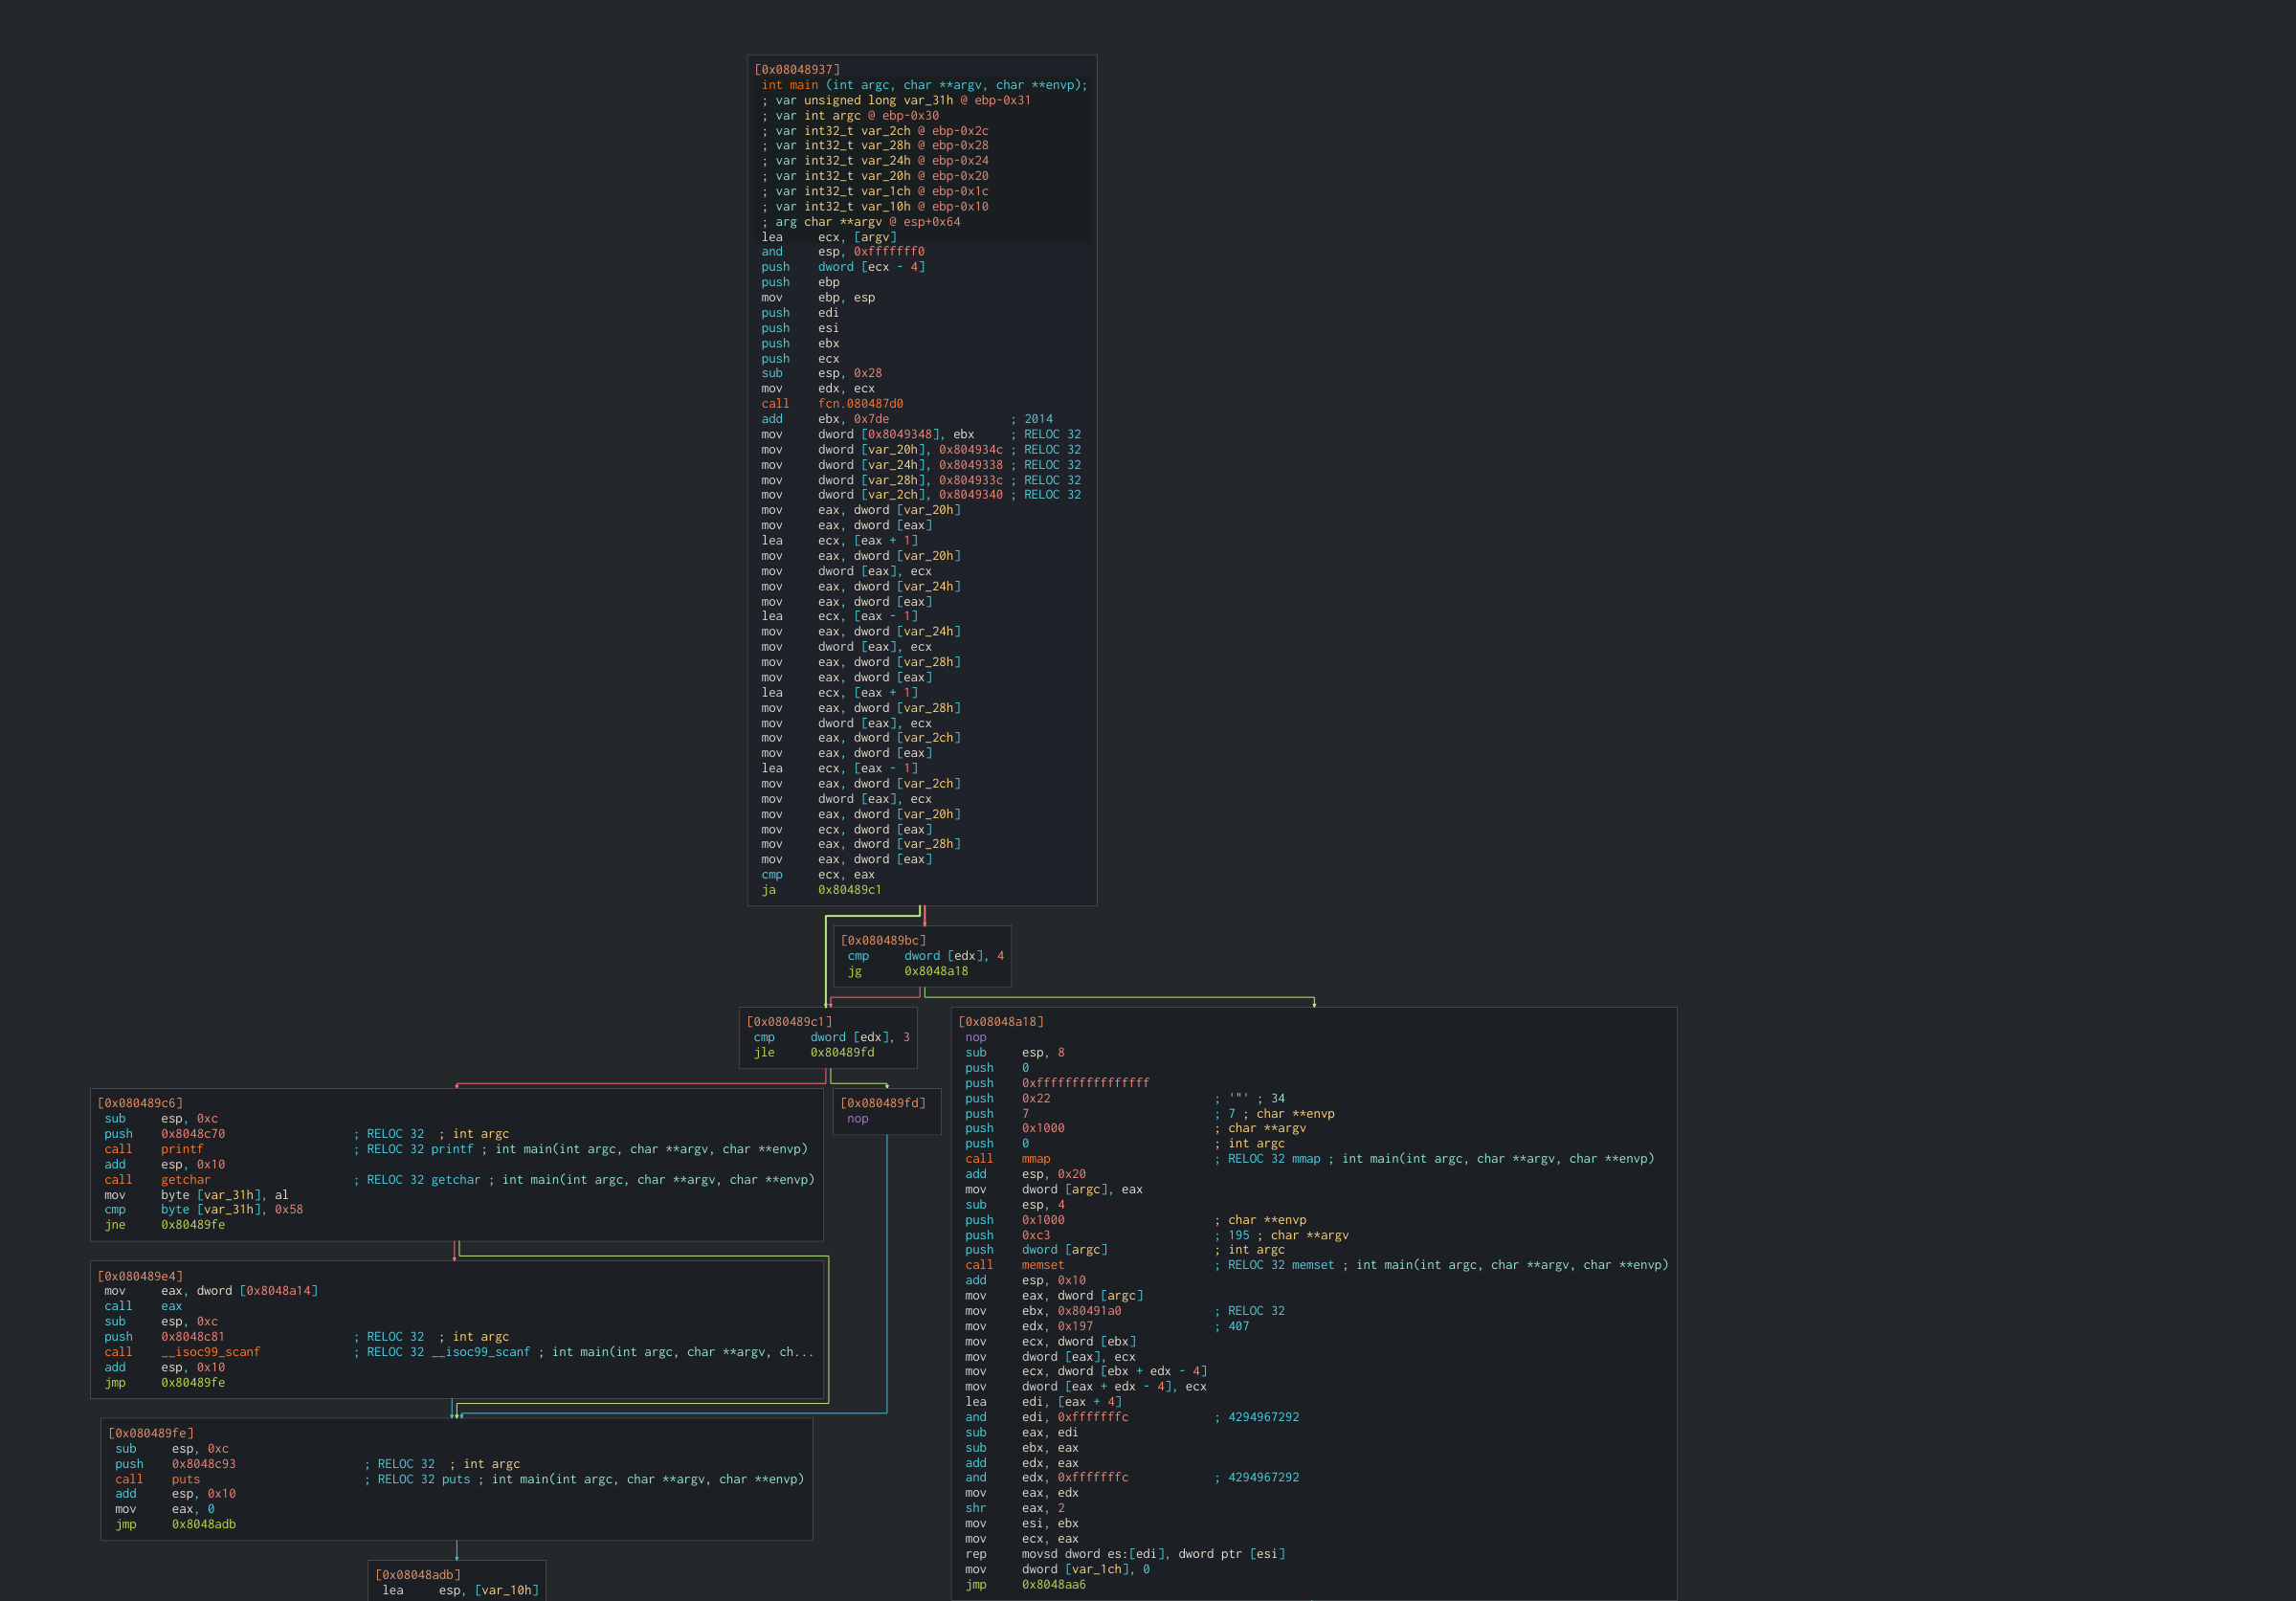
\includegraphics[width=.9\linewidth]{bombs_landed_main_branches.png}
\caption{\label{fig-main-branches}Two exclusive branches}
\end{figure}
These two main branches can be seen on \hyperref[fig-main-branches]{Figure}.
The selection of the branch depends on the number of arguments passed to the program. If the count of arguments equals to three left branch will be selected. If the arguments count equals to 4 the righ branch is chosen.
I did spent many time in the left branch as I thought it would be somehow important. The left branch can be seen on \hyperref[fig-left-branch]{Figure}. Firstly, there is prompting for input via the getchar call and then there is check for the first character of the given string. The check is for the 'X' letter, if the condiction succeed the program will call some address. But as much as I tried the calling address did not changed and at all and every attempts ended up as segmentation fault.
\begin{figure}[htbp]
\centering
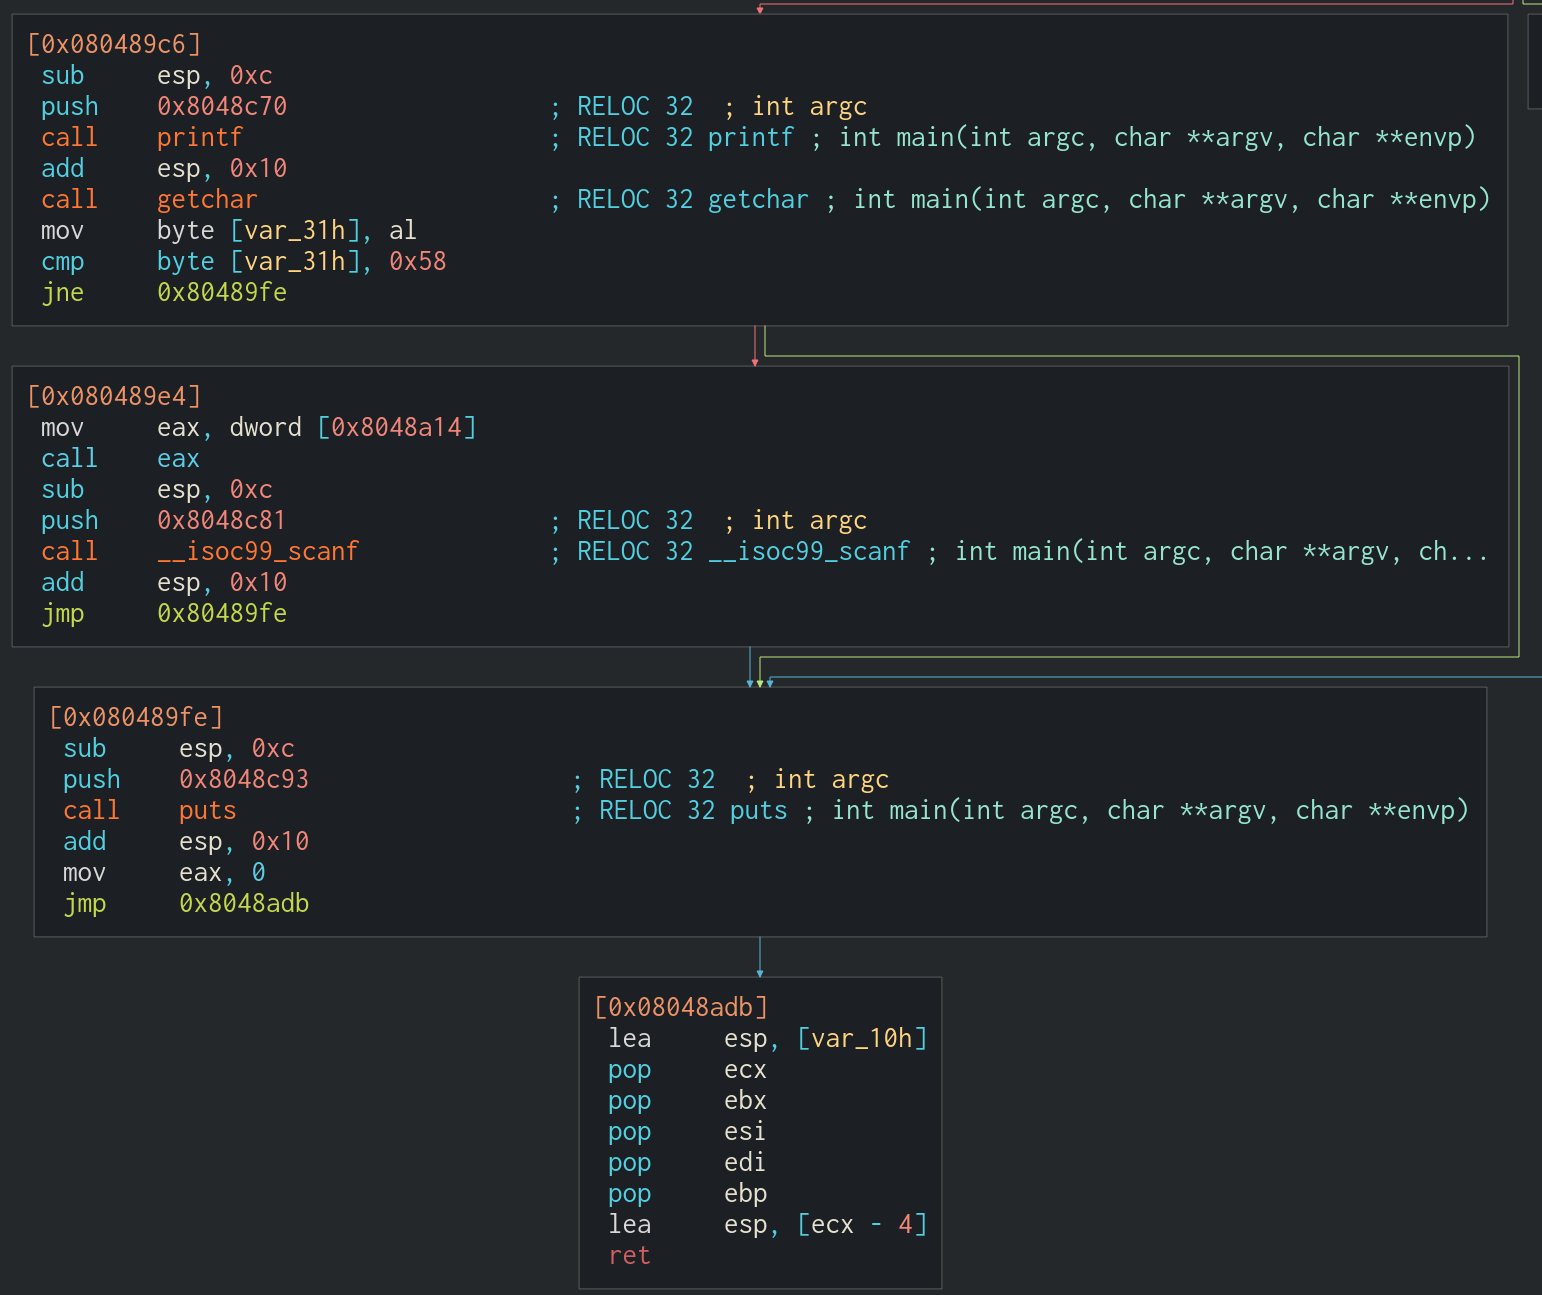
\includegraphics[width=.9\linewidth]{boms_landed_left.png}
\caption{\label{fig-left-branch}Left branch}
\end{figure}

I decided to move to the right branch after quite time spent in left. The right branch from first look seemed to be doing some calculation and memory writting but nothing straightforward that could be seen without evaluation.
The calculation and memory write of right branch is on the \hyperref[fig-main-branches]{Figure}. The most interesting was there was call to that newly written memory. Once I launched the debugger in cutter, hit breakpoint at the call and start stepping stepping arround, it was obvious the newly written data was dynamicly generated code. The decompiled function in cutter is on the \hyperref[fig-dynamic]{Figure}.
\begin{figure}[htbp]
\centering
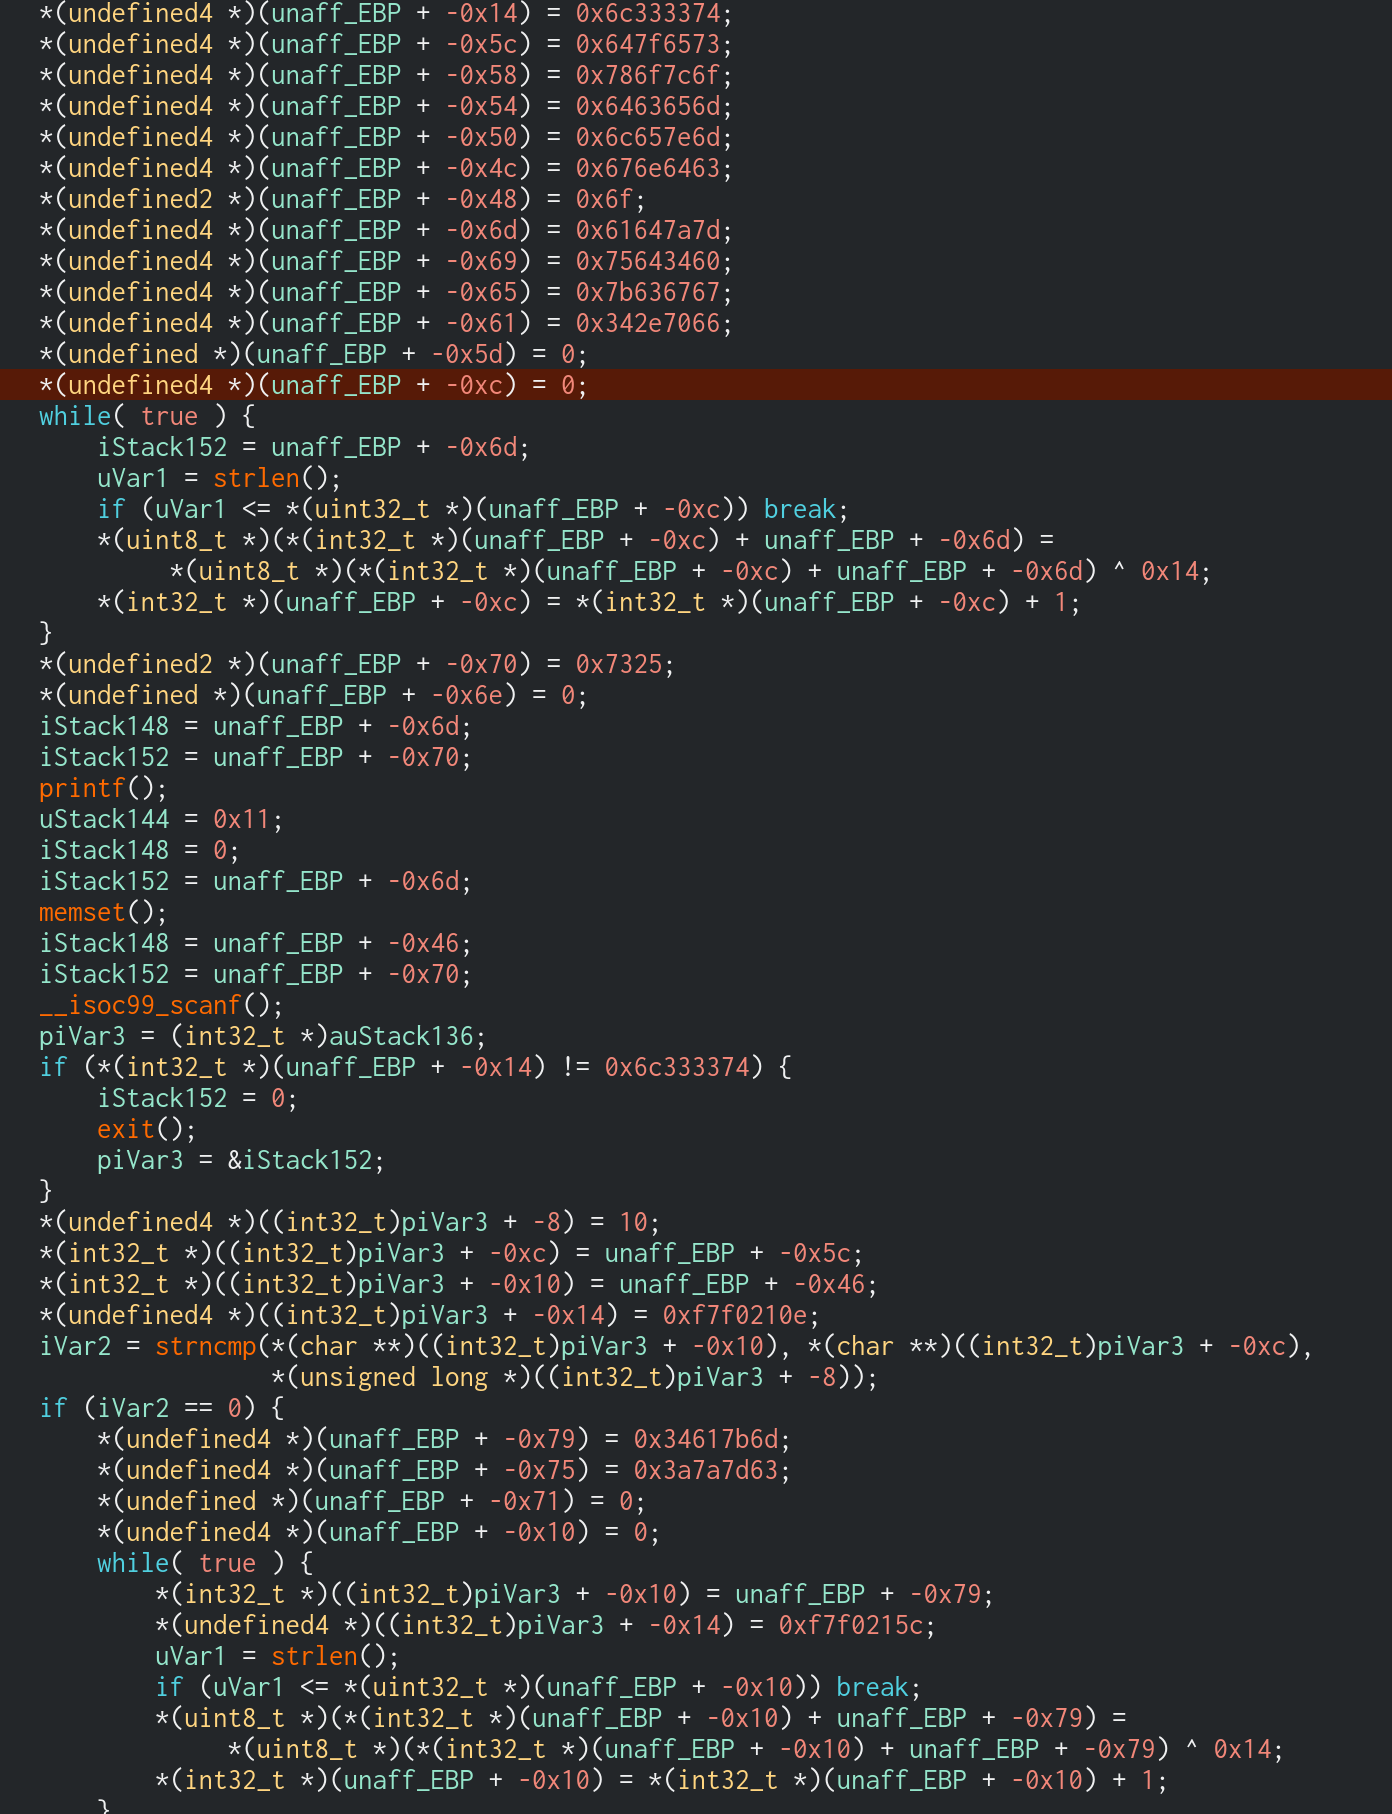
\includegraphics[width=.9\linewidth]{boms_landed_new_function.png}
\caption{\label{fig-dynamic}Dynamically generated code}
\end{figure}

After thorough inspection, this newly generated code does prompt for input via scanf and then use strncmp to compare two strings. When I provided the exact same input as the strncmp was checking against it failed, which was weird. At this point, I did not known what to do with the failing strncmp as the inputs were same but it was returning non-zero code anyway. I stumbled around LD PRELOAD technique, on the internet that could help me with debugging strncmp.
The aim of this technique is to replace any function with help of linker that is dynamically loaded from the shared libraries, typical example is the functions from libc library. As the binary is not statically compiled and was using shared libraries this was possible.
The newly created strncmp looked like this and it yield the string that is compared against.

\begin{verbatim}
#define _GNU_SOURCE
#include <dlfcn.h>
#include <stdio.h>
#include <string.h>

 // Define an alternative name for strcmp()
 int (*orig_strncmp)(const char *str1, const char *str2, size_t n);

 int strncmp(const char *str1, const char *str2, size_t n) {
    // Backup the orginal call to strcmp() in orig_strcmp()
    // by initialazing the pointer of orig_strcmp().
    if(!orig_strncmp) orig_strncmp = dlsym(RTLD_NEXT, "strncmp");
    printf("You should try '%s'\n", str2);

    // return the proper result of strcmp()
    return orig_strncmp(str1,str2,n);
 }
\end{verbatim}

This C code has to be compiled as shared library object and passed to the linker with help of env variable during running the binary, this is shown in below bash code.
\begin{verbatim}
#The m32 stands for 32-bit architecture
#Other flags serve for shared-library compilation
gcc -fPIC -shared -m32 preload_strcmp.c -o preload_strcmp.so

LD_PRELOAD=./preload_strcmp.so ./BombsLanded 1 2 3 4
\end{verbatim}

To my surprise this technique did yield the correct password. This got me wonder why there is different string in strncmp during debugging. As I foudn out, the system strncmp is called but its called from the program modified strncmp but their both names are exactly same, so the author of challenge known that the user will not bother checking the system functions and looks only on the non-familliar ones.
\begin{figure}[htbp]
\centering
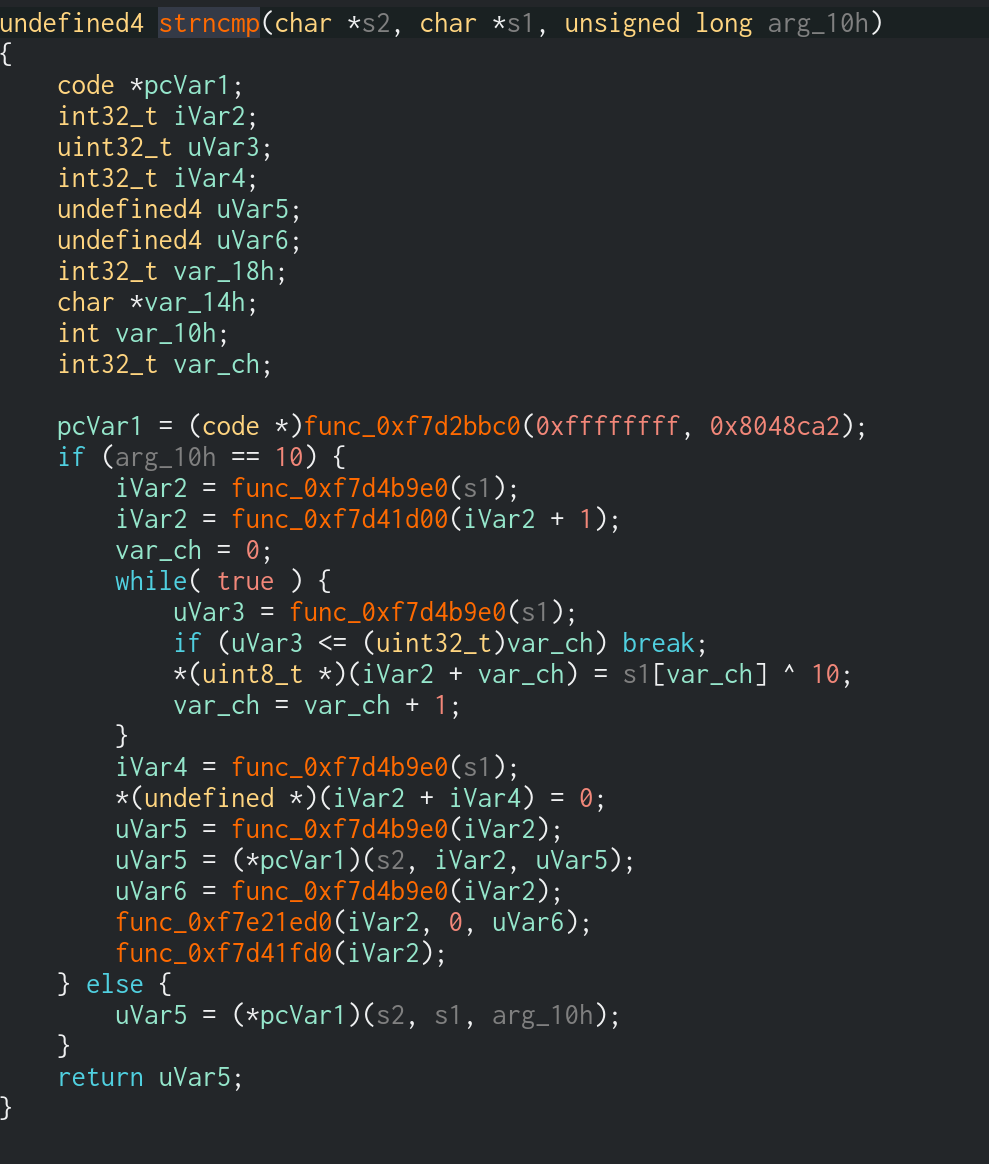
\includegraphics[width=.9\linewidth]{bombs_landed_strcmp.png}
\caption{\label{fig-strncmp}Program custom strncmp}
\end{figure}
The program decompiled strncmp is at \hyperref[fig-strncmp]{Figure}.
So now we can see that the program strncmp is calling system strncmp but in case the string has length 10 it will be xored with 10 firstly and then compared. That was the reason why my input, which was same as it was checked againts was not working.
\section{Simple Keygen}
\label{sec:org17752d0}
Object of this challenge was to generate correct password. This challenge was simple and pretty much straightforward.
The only custom function called by main was function named usage. The decompiled usage fuction is on \hyperref[fig-simple-usage]{Figure}.
\begin{figure}[htbp]
\centering
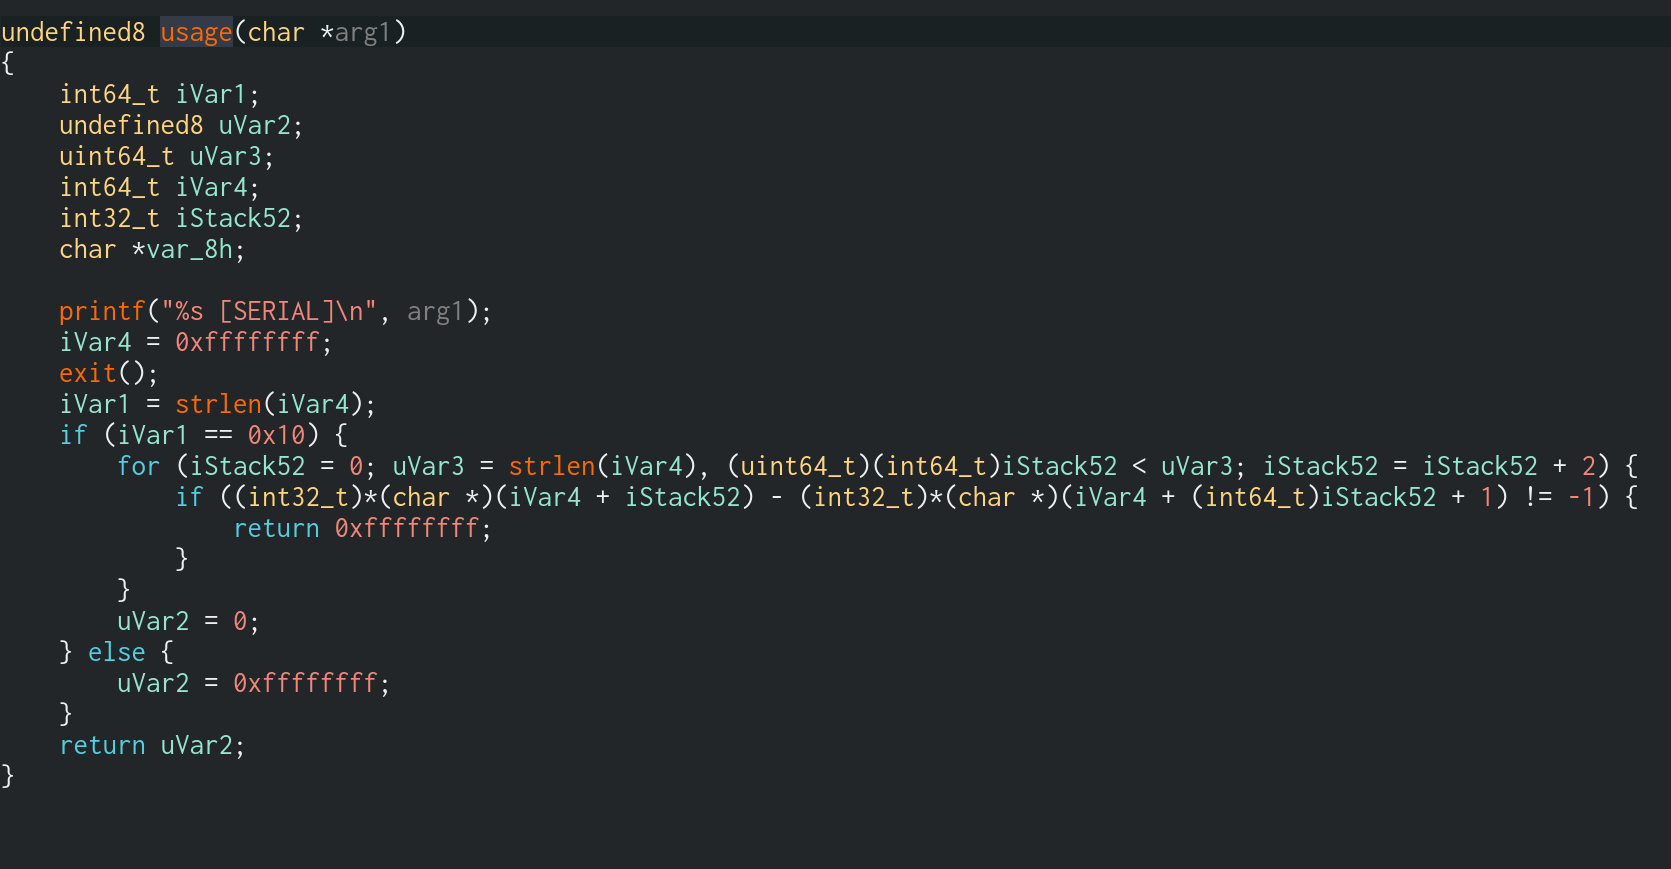
\includegraphics[width=.9\linewidth]{simple_keygen.png}
\caption{\label{fig-simple-usage}Usage function}
\end{figure}

So according the usage function, the given password has to meet two conditions. First is the length should be equal to 16 or 0x10 in hexadecimal.
The second condition is that each character on even index had to have the ordinal value lower by one from its neighbouring character that right on the right side of him.
So for example, the string 'abcdefghijklmnop' is good password as it has sufficient length and every character pair is meeting the condition that left character is one lower than right character in ordinal value.
The ordinal difference between characters in python is shown below.
\begin{verbatim}
ord('a') - ord('b') == -1
ord('c') - ord('d') == -1
ord('e') - ord('f') == -1
\end{verbatim}
According the conditions, the characters can repeat so the 'abababababababab' string is valid as well.
\section{rop-obf}
\label{sec:orgefbd3d7}
The object of this challenge was to find another correct input and the program should then print '1' instead of
'0'. There is no function that could be properly decompiled in whole binary. This is due to natur of used obfuscated technique. The example of binary code is on \hyperref[fig-rop-entry]{Figure}.
\begin{figure}[htbp]
\centering
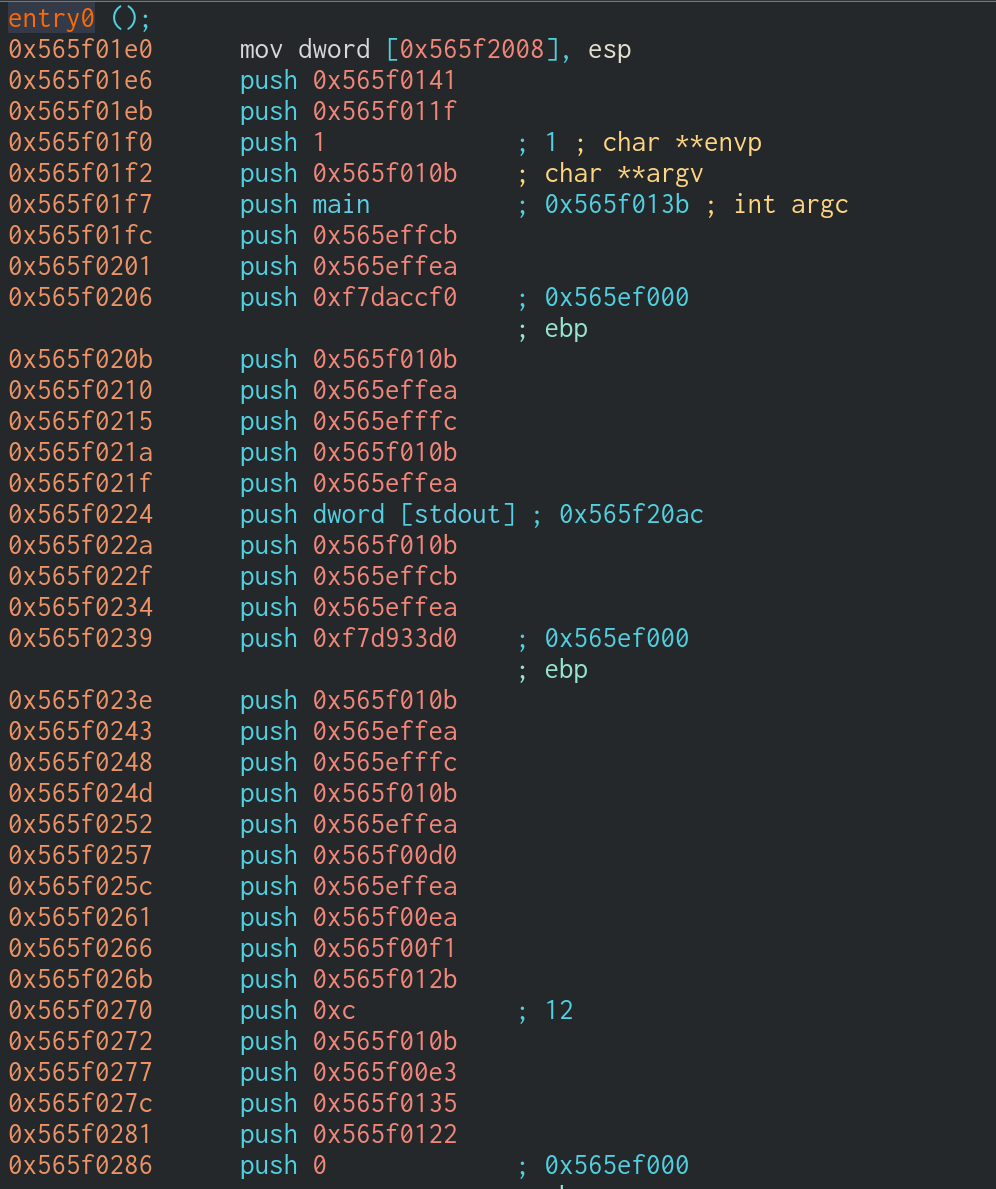
\includegraphics[width=.9\linewidth]{rop_obf.png}
\caption{\label{fig-rop-entry}rop-obf obfuscation}
\end{figure}

As the code suggets, the name stand for return-orietended programming (rop) obfuscation (obf). This means that obfuscation is based on using the \texttt{ret} assembler instruction, which pops the value from stack and put it to the instruction pointer which shows the next executed instruction. Firstly, the whole program is pushed into the stack in the entry function as shown in \hyperref[fig-rop-entry]{Figure} and first \texttt{ret} instruction is starting it. The only system used system function is for the reading \texttt{STDIN} but nothing with string comparison as strcmp where I could use the LD PRELOAD technique mentioned in BombsLanded.
I did tried few random inputs and the program took always 6 inputs, so there will probable be six comparisons.
\begin{figure}[htbp]
\centering
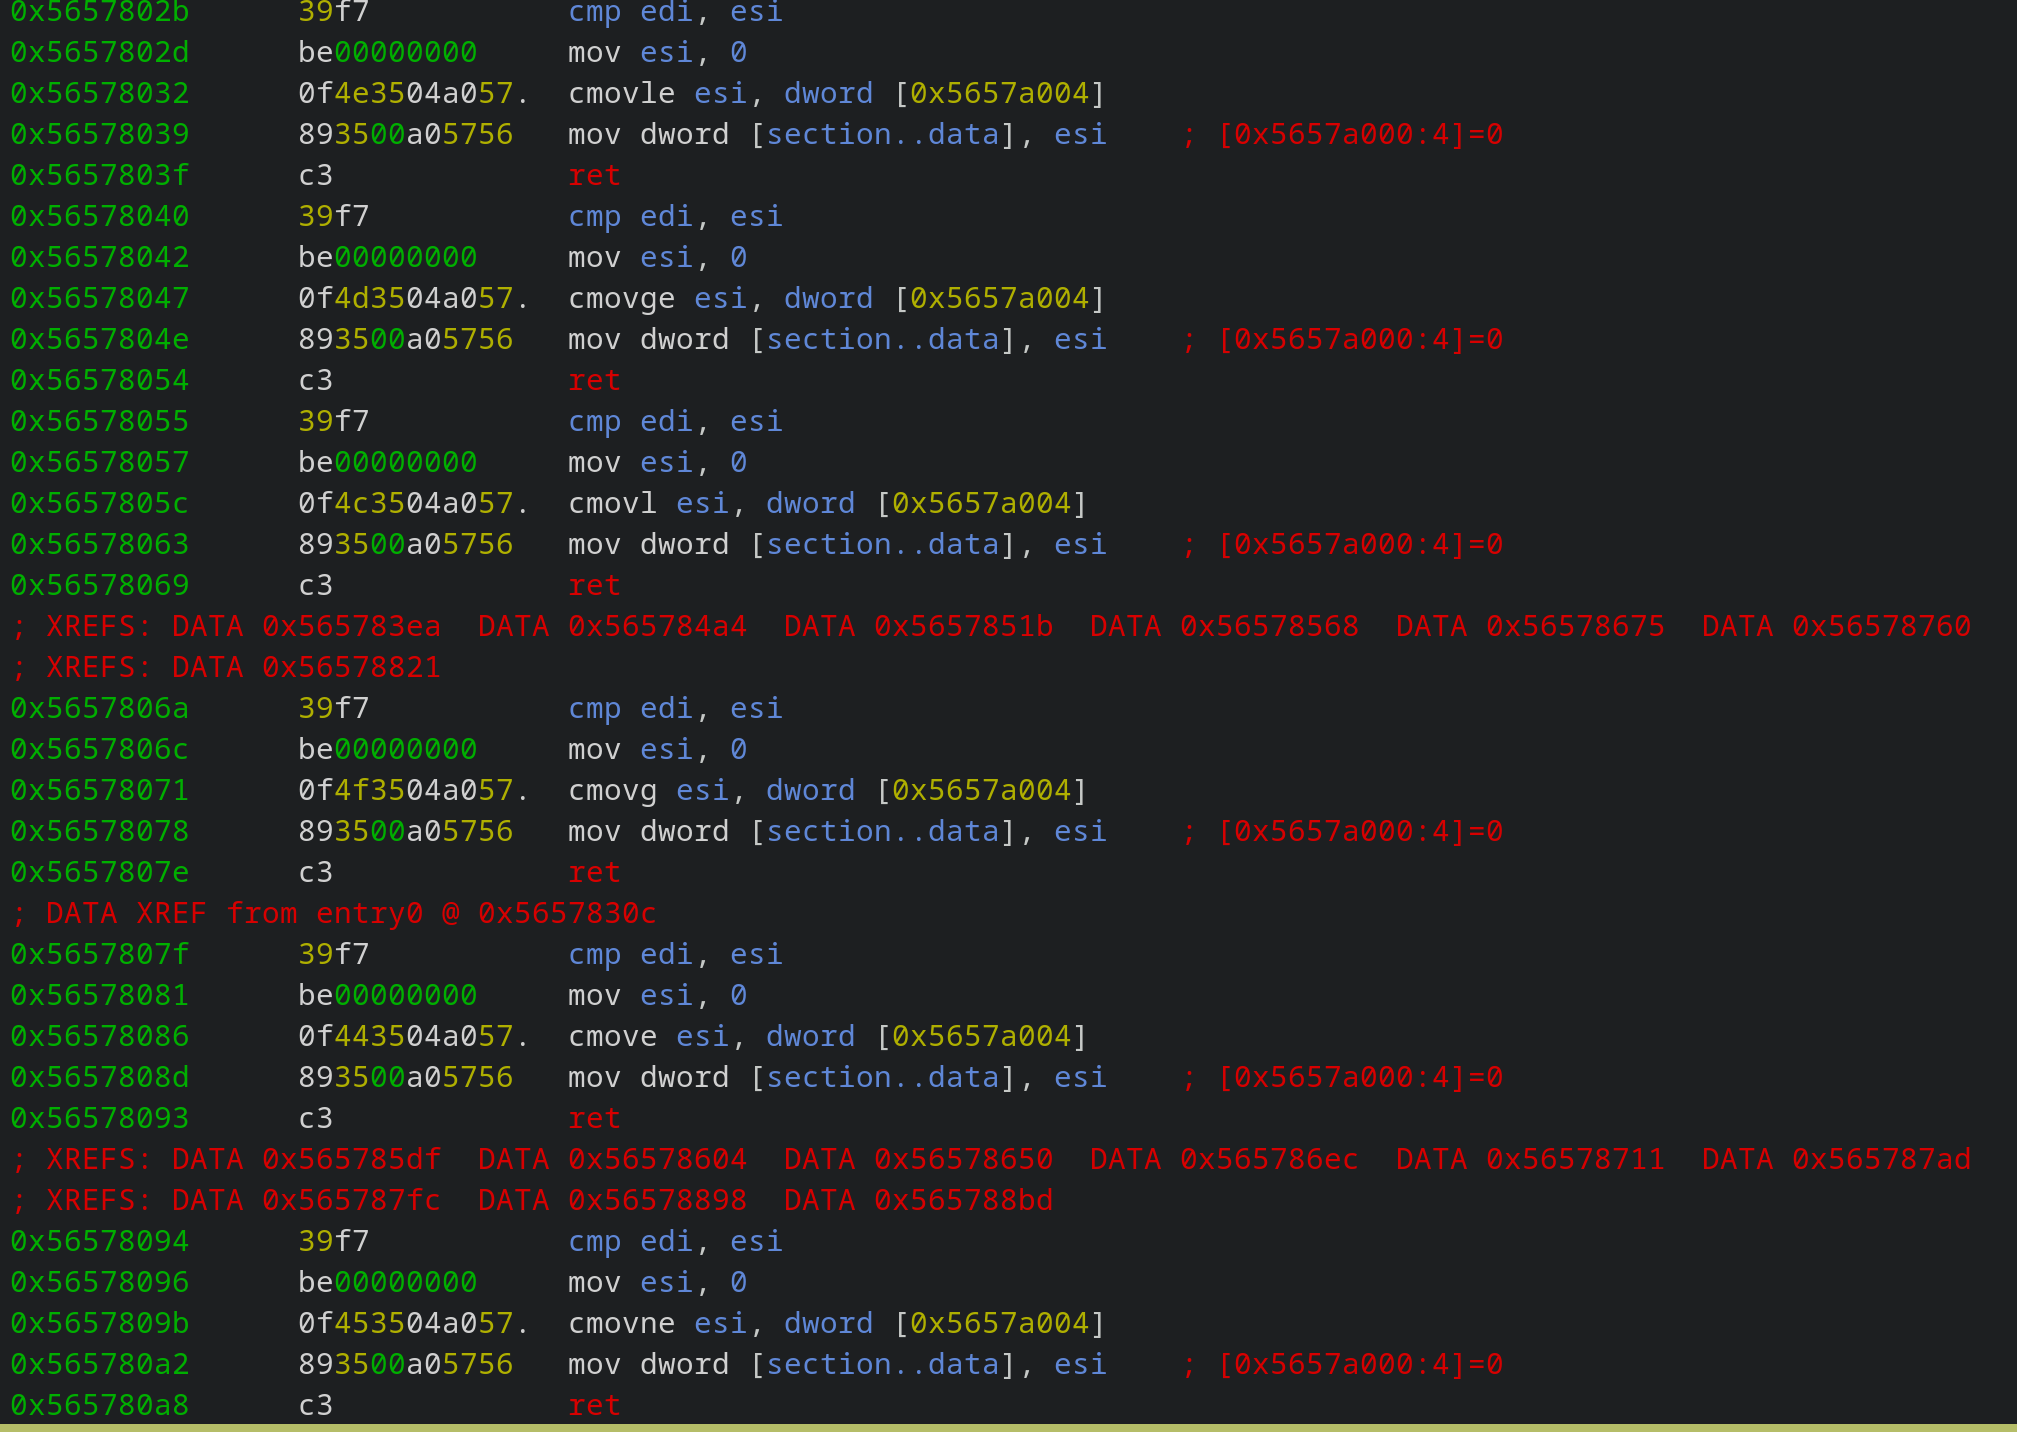
\includegraphics[width=.9\linewidth]{simple_cmp.png}
\caption{\label{fig-cmp}CMP instructions references}
\end{figure}

So the input comparison should be done with \texttt{cmp} instruction. With the help of radare2 and its reference finding, there are six \texttt{cmp} instructions and only 3 of these are used because there are referenced by some \texttt{push} instruction. The mentioned \texttt{cmp} instructions and references are on \hyperref[fig-cmp]{Figure}. I put breakpoints on the referenced \texttt{cmp} instructions and as I was stepping through code, the input was firstly xored with some value and then compared with correct input. So I knew what should be the correct output after xor then let some CSP solver do the work. The simple code below shows the solution in python with help of z3-solver.

\begin{verbatim}
from z3 import *
s=Solver()
array=[BitVec("array%i"%i,32) for i in range(6)]

s.add(array[0]^0x83==0x87)
s.add(array[1]^0x36==0x3e)
s.add(array[2]^0x9d==0x92)
s.add(array[3]^0xcd==0xdd)
s.add(array[4]^0xec==0xfb)
s.add(array[5]^0xf6==0xdc)

if s.check()==sat:
    flag=s.model()
    for i in range(6):
        ans=((flag[array[i]]))
        print(ans)
\end{verbatim}

And with help of script we have our solution as 4,8,15,16,23,42 which prints '1'.
\end{document}
